\documentclass[a4paper]{article}

\usepackage[czech]{babel} %https://github.com/michal-h21/biblatex-iso690
\usepackage[
   backend=biber      % if we want unicode 
  ,style=iso-numeric % or iso-numeric for numeric citation method          
  ,babel=other        % to support multiple languages in bibliography
  ,sortlocale=cs_CZ   % locale of main language, it is for sorting
  ,bibencoding=UTF8   % this is necessary only if bibliography file is in different encoding than main document
]{biblatex}

\usepackage[utf8]{inputenc}
\usepackage{fancyhdr}
\usepackage{amsmath}
\usepackage{amssymb}
\usepackage[left=2cm,right=2cm,top=2.5cm,bottom=2.5cm]{geometry}
\usepackage{graphicx}
\usepackage{pdfpages}
\usepackage{url}
\usepackage{bm}

\usepackage{siunitx}
\sisetup{locale = DE}  %, separate-uncertainty = true    kdybych chtel +/-

\usepackage{float}
\newfloat{graph}{htbp}{grp}
\floatname{graph}{Graf}
\newfloat{tabulka}{htbp}{tbl}
\floatname{tabulka}{Tabulka}

\renewcommand{\thefootnote}{\roman{footnote}}

\pagestyle{fancy}
\lhead{Praktikum IV - (A10) Pulzní metoda NMR (část základní)}
\rhead{Vladislav Wohlrath}
\author{Vladislav Wohlrath}

\bibliography{source}

\begin{document}

\begin{titlepage}
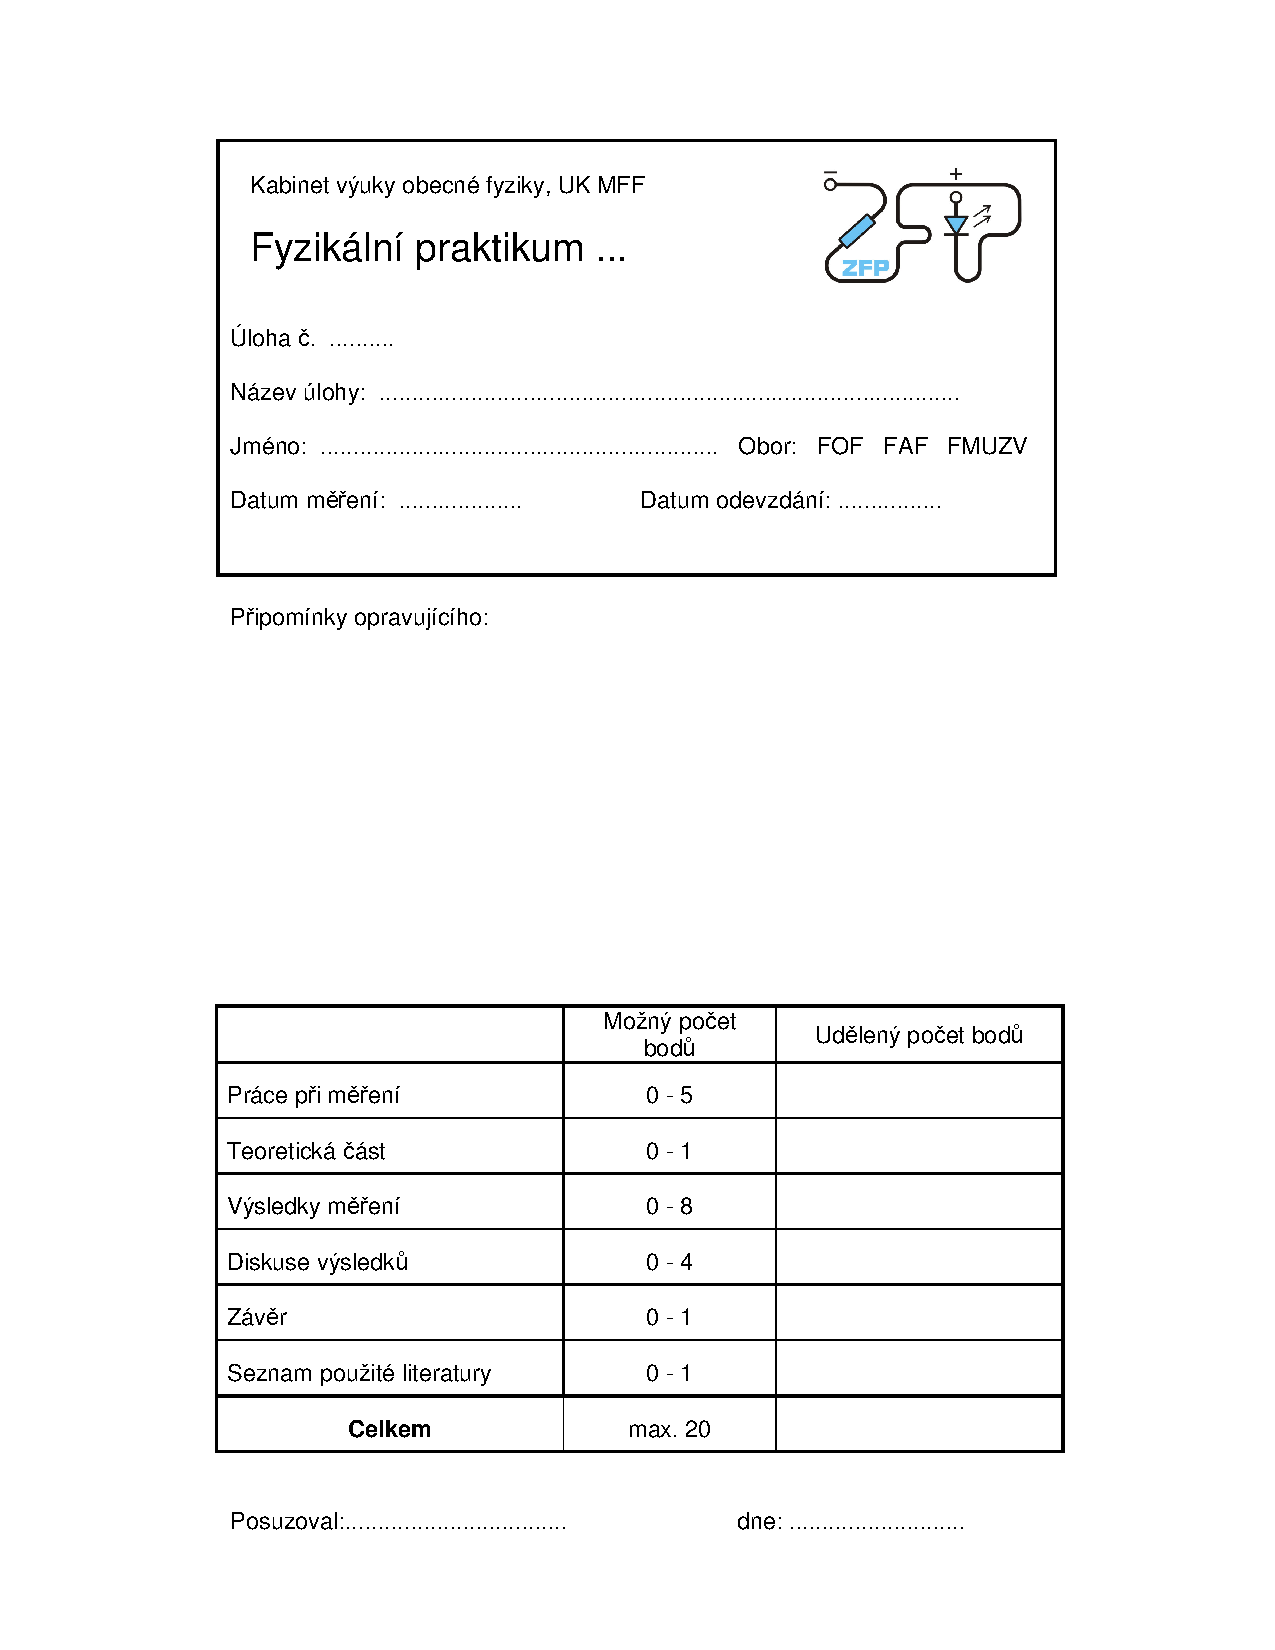
\includepdf[pages={1}]{./graficos/titlelist.pdf}
\end{titlepage}

\section*{Pracovní úkoly}
\begin{enumerate}
\item Nastavení optimálních excitačních podmínek signálu FID $^1$H ve vzorku pryže.
\item Měření závislosti amplitudy signálu FID $^1$H ve vzorku pryže na délce excitačního pulzu. Určení velikosti amplitudy radiofrekvenčního pole $B_1$.
\item Studium signálu dvouimpulzového spinového echa $^1$H ve vzorku pryže.
\item Studium procesu koherentní sumace.
\end{enumerate}

%Teoretická část
\section*{Teoretická část}
Proton má magnetický moment
\begin{equation}
\bm{\mu}=\gamma\bm{I}\,,
\end{equation}
kde $\gamma$ je gyromagnetický poměr a $\bm{I}$ je jeho celkový moment hybnosti.
Pokud proton umístíme do magnetického pole velikosti $B_0$ ve směru osy $z$, bude magnetický moment protonu vykonávat \emph{Larmorovu precesi} s Larmorovvou frekvencí \cite{skripta}
\begin{equation} \label{e:fL}
f_L=\frac{\gamma B_0}{2\pi} \,.
\end{equation}

Označíme $\bm{M}$ jádernou magnetizaci.
V látce bude atom interagovat i s okolními atomy a jeho magnetický moment se bude stáčet do směru vnějšího magnetického pole. Pokud jsou magnetické momenty před časem $t=0$ orientované náhodně (žádné vnější pole, $\bm{M}=0$), a v čase $t=0$ zapneme magnetické pole, bude časový vývoj magnetizace (složky $z$) dán \cite{skripta}
\begin{equation} \label{e:mz}
M_z(t)=M_0 (1-\exp(-t/T_1)) \,,
\end{equation}
kde $M_0$ je rovnovážná magnetizace v daném poli a $T_1$ je tzv. spin-mřížková relaxační doba.

Pokud v čase $t=0$ byla naopak příčná složka $M_t$ rovna hodnotě $M_{t0}$, pak pro její vývoj v čase platí \cite{skripta}
\begin{equation} \label{e:mt}
M_t(t)=M_{t0} \exp(-t/T_2) \,,
\end{equation}
kde $T_2$ je tzv. spin-spinová relaxační doba. Příčná složka bude zanikat kvůli jak kvůli stáčení momentů do směru pole, tak kvůli nepatrně rozdílným Larmorovým frekvencím jednotlivých jader (nehomogenní pole).

Počáteční magnetizaci vybudíme polem $\bm{B_0}$. Za trigrovací dobu $T_0$ pustíme krátký harmonickým pulz ve směru osy $x$ s amplitudou $B_1$, frekvencí $f_L$ a délkou $\tau$. Tím otočíme magnetizaci okolo osy $x$ o úhel \cite{skripta}
\begin{equation} \label{e:uhel}
\varphi=\omega_1\tau=\gamma B_1 \tau \,.
\end{equation}
Volíme takové $\tau$, aby $\varphi=\pi/2$ ($\pi/2$-pulz). Magnetický moment je potom ve směru osy $y$.

Magnetizace se poté stáčí do směru pole $\bm{B_0}$ a my pozorujeme tzv. signál volné precese (FID), který je Fourierovým obrazem spektra NMR.

Po určité době dojde k utlumení FID signálu vlivem nehomogenního pole dojde k rozfázování jednotlivých momentů s různou $f_L$. Pokud nyní (po době $t_{12})$ od prvního $\pi/2$-pulzu) pustíme $\pi$-pulz, dojde po době $t_{12}$ k jejich opětovnému sfázování. Tomuto jevu říkáme spinové echo.

Standardní odchylka šumového napětí je
\begin{equation}
\sigma^2_{\bar{u^n}}=\sqrt{\frac{1}{L-1} \sum_{i=1}^{L} (\bar{u^n_i})^2  } \,,
\end{equation}
kde $\bar{u^n_i}$ je hodnota šumu v jednotlivých kanálech a $L$ je počet použitých kanálů. Pokud $u^n_i $ bude aritmetický průměr $N$ náhodných veličin se standardní odchylkou $\sigma_{u^n}$, pak bude díky centrální limitní větě platit \cite{skripta}
\begin{equation}
\sigma^2_{\bar{u^n}} \approx \frac{\sigma_{u^n}}{\sqrt{N}} \,.
\end{equation}

%Výsledky měření
\section*{Výsledky měření}

%Diskuze výsledků
\section*{Diskuze}

Závislosti na grafech \ref{g:t1} a \ref{g:tau} se velmi dobře shodují s teoretickými.
Naopak závislost na grafu \ref{g:t2} neodpovídá příliš přesně exponenciálnímu poklesu u vyšších časů.

Nejistotu u časů $T_1$ a $T_2$ považujeme za podhodnocenou, pokud například závislost na grafu \ref{g:t2} fitujeme (lineárně) až po zlogaritmování (což odpovídá přiřazení váhy bodům), dostaneme hodnotu \SI{1600}{\us}. Proto jsme v závěru nejistotu patřičně zvětšili a nejistota uvedená v části \emph{Výsledky měření} je pouze statistická chyba fitu.

Největší chybu metody způsobuje pravděpodobně nehomogenita pole, která je řádově vyšší než je u podobných přístrojů běžné.

Intenzita šumu klesá úměrně $1/\sqrt{N}$. Pro $N=200$ už je šum poměrně zanedbatelný.

%Závěr
\section*{Závěr}
Určili jsme spin-mřížkovou a spin-spinovou relaxační dobu (viz \emph{Diskuze}),
\begin{equation*}
T_1=\SI{65(10)}{\ms}  \,,\qquad \qquad T_2=\SI{1000(300)}{\us} \,.
\end{equation*}
Určili jsme amplitudu radiofrekvenčního pole
\begin{equation*}
B_1=\SI{1.076(3)}{\milli\tesla} \,.
\end{equation*}

Při středování více průběhů dochází ke zvýšení poměru signálu ku šumu. Intenzita šumu klesá poměrně přesně jako $1/\sqrt{N}$.


\printbibliography[title={Seznam použité literatury}]

\end{document}